\section{Decorating Sequences}
\label{sec:Decorating Sequences}
This chapter explores how to modify Sequences by implementing the Decorator 
Pattern and effectively managing Sequence state. And then we will discover 
powerful techniques to enhance Sequence functionality and manipulate data.

\subsection{Decorator Pattern}
\label{sub:Decorator Pattern}
Let us look at the Decorator Pattern~\cite[p.~226]{gang_of_four_depa} to understand the content of the 
following sections. In object-oriented programming, the Decorator Pattern is a 
widely used concept. An object decorates another, as the name implies. As a 
result, an outer object holds an inner object, while both implement the same 
interface. The outer object forwards requests to the inner one. This enables
the outer to modify (decorate) the behavior of the inner. 
Figure \ref{fig:seq_diagramm} shows how a decorator forwards the receiving calls and 
transfers the answer back to the client.

% TODO: replace
\begin{figure}[H]
    \centering
    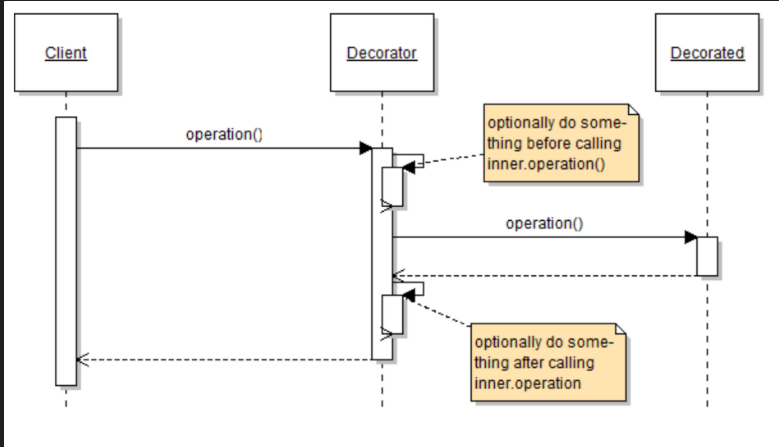
\includegraphics[width=0.8\textwidth]{./mainmatter/pictures/decorator_sequence_diagramm.png}
    \caption{Decorator Patter Sequence Diagram}
    \label{fig:seq_diagramm}
\end{figure}

The Decorator Pattern is often used in object-oriented programming languages 
because of its ability to add functionality to an object at runtime. It is also 
possible to add extended functionality to a single class object. In the 
following, we will see how to exploit this to manipulate and change an Iterable.

\subsection{Processing Sequences}
\label{sec:Processing Sequences}
We use precisely that decorating approach to process Iterables further. 
The goal is to find a way to manipulate sequences so that they can solve 
complex problems. With many other programming languages, it is possible to write 
programs this way. Lists and operations on lists solve numerous problems in 
computer science. This way of programming has the advantage that the structure 
of the code is declarative. This code is more straightforward to understand 
and easier to extend.

\subsubsection{Processing Iteratbles with Functions}
\label{subsub:Processing Iterables with Functions}
In the following, |map| serves as a representative for any function of the
Sequence Library. We call such functions in the following operators,
according to the package they are in.
Listing~\ref{lst:impl_map} shows how |map| processes a Sequence. The 
implementation use the Decorator approach just mentioned. |map| decorates a
|Sequence| on line~\ref{line:obj_mapped}.
\newline
On line~\ref{line:args}, the function signature shows that a client can invoke 
|map| with two arguments:

\begin{enumerate}
  \item{A mapper-function capable of processing an element of an |Iterable|}
  \item{An |Iterable|}
\end{enumerate}

An iterable must adhere to the JS iteration protocol 
outlined in Section~\ref{subsub:The Iterable Protocol}. Therefore, |map| can 
process Sequences, Arrays, or any other iterable. 

\begin{lstlisting}[
  style=ES6, 
  caption=Implementation of map,
  label={lst:impl_map}
  ]
const map = mapper => iterable => { *'\label{line:args}'*
*'\label{line:state_iterable}'*
const mapIterator = () => {
   const inner = iteratorOf(iterable);*'\label{line:state_iterator}'*
   let mappedValue;
 
   const next = () => {
     const { done, value } = inner.next();*'\label{line:inner_next}'*
     if (!done) mappedValue = mapper(value);
 
     return { /**@type boolean */ done, value: mappedValue }
   };
 
   return { next };
  };
 
  return createMonadicSequence(mapIterator);
};

const sequence = Sequence(0, x => x < 10, x => x++);*'\label{line:seq_definition}'*
const mapped   = map(x => x * 2)(sequence);*'\label{line:obj_mapped}'*
\end{lstlisting}

Because |map| decorates iterables, |map| also returns an object adhering JS
iteration protocols. 
We define this object on line~\ref{line:obj_mapped} as |mapped|. 
Consequently, |map| also has a next function. Since the JS iteration protocol 
specifies only this single function, it is the only one that must be externally 
callable. The object |mapped| forwards function calls on |next| to the
inner function |next|, on line~\ref{line:inner_next}. The |mapper| function then 
processes the result and returns it. so |map| decorates the function |next| of
the inner |Iterable|.

\subsection{Benefits of the Decorator Approach}
\label{sub:Benefits of the Decorator Approach}
This section discusses the benefits and consequences of using the Decorator 
Pattern to implement the Sequence Library. We start with the fact that functions 
stand-alone, then discuss the options for managing State.

\subsubsection{Stand-alone Functions}
\label{subsub:Standalone Functions}
In an object-oriented approach, the |Sequence| object would provide a function
|map|. Therefore, such operators are available by using dot notation,
similar to Java implements the Stream API \cite{java_stream}. 
However, with the approach of providing independent functions, there 
are three significant advantages:

\begin{enumerate}
  \item {Strict adherence to the open-close principle~\cite[p.~3]{eilebrecht_patterns_2019}. Changes to an operator do
      not affect the implementation of Sequence. Also, extensions to the 
      Sequence Library do not affect existing code.
    }
  \item{Adherence to the single responsibility approach. The Sequence 
      constructor has only the task of creating a sequence. Mapping the
    elements of a sequence is not its responsibility.
  }
  \item{Easy scalability is guaranteed. It is very straightforward to add new 
    functionality from the outside.
  }
\end{enumerate}

Since the independent implementation of the iterable operators, the last
argument is the iterable object. The operator defines the 
parameters in a curried style. So it is possible to benefit from eta-reduction 
in different situations.

\subsubsection{Stateful Decorating}
\label{subsub:Stateful Decorating}
A state is present as soon as operators decorate iterables or implement 
additional functionalities. This chapter explores the implementation of state
within operators and the implications it involves.

There are two valid possibilities for including state.
The first Scenario places the state into the closure scope to the surrounding 
operator of the iterator. The second Scenario implements the state into the 
closure scope of the iterator. In both variants, it is crucial to ensure that 
the underlying object remains unchanged.

\subsubsection{Scenario 1}
\label{subsub:Scenario 1}
Listing~\ref{lst:scen_1} shows an example of a Sequence generating numbers from
zero to five. On line ~\ref{line:scen_1_state}, value |i| works as a counter 
and represents the state. 
A call to |SampleIterator| creates a state which is valid for the entire 
object's lifetime.

\begin{lstlisting}[
  style=ES6, 
  caption=Scenario 1 - State in closure scope of iterable,
  label={lst:scen_1}
  ]
const SampleIterable = () => {

  let i = 0; *'\label{line:scen_1_state}'*
  const next = () => {
    return { done: i > 5, value: i++ };
  };

  return { [Symbol.iterator]: () => ({ next }) }
};
\end{lstlisting}

Listing~\ref{lst:scen_1_demo} shows a possible program flow. 
The program first creates an object of |SampleIterator|, maps it and processes
an element on the original object. Note, that on line~\ref{line:scen1_map} |map| also 
uses the same |Iterable|. Line~\ref{line:scen1_output} shows an expected result.

\begin{lstlisting}[
  style=ES6, 
  caption=Scenario 1 - Example usage,
  label={lst:scen_1_demo}
  ]
const seq = SampleIterable(0, x => x < 5, x => x++); // [0, 1, 2, 3, 4]
const mapped = map(id)(seq); *'\label{line:scen1_map}'*

for (const elem of mapped) {
  console.log(elem);
  break; // Just consuming one element
}
// => Logs: '0'

for (const elem of seq) {
  console.log(elem);
}
// => Logs: '[0, 1, 2, 3, 4]' *'\label{line:scen1_output}'*
\end{lstlisting}

To achieve the expected result, |map| must copy the object before processing.
That implies that each |Iterable| must be copyable. An example implementation
of a copyable |Iterable| shows Listing~\ref{lst:iterable_with_copy}.

\begin{lstlisting}[
  style=ES6, 
  caption=Iterable with copy,
  label={lst:iterable_with_copy}
  ]
const SampleIterable = () => {

  let i = 0;
  const next = () => {
    return { done: i > 5, value: i++ };
  };

  const copy = () => SampleIterable();

  return {
    [Symbol.iterator]: () => ({ next }),
    copy: copy *'\label{line:iterable_copy}'*
  }
};
\end{lstlisting}
Since |copy| must be callable from outside, it requires returning it alongside 
|[Symbol.iterator]| on line~\ref{line:iterable_copy} . |map| is now
able to copy the underlying  |Iterable| before consuming the elements.
However, |map| itself must also implement |copy|, because its interface must be
the same as the decorated object. The following Listing~\ref{lst:map_with_copy} 
shows an implementation of |map| supporting copy.

\begin{lstlisting}[
  style=ES6, 
  caption=Implementation of map with copy,
  label={lst:map_with_copy}
  ]
const map = mapper => iterator => {
 const inner = iterator.copy();*'\label{line:copy_of_inner}'*
 let mappedValue;

 const next = () => {
   const { done, value } = inner[Symbol.iterator]().next();*'\label{line:consuming_inner}'*
   if (!done) mappedValue = mapper(value);
   return { done, value: mappedValue }
 };

 return {
   [Symbol.iterator]: () => ({ next }),
   copy: () => map(mapper)(inner*'\label{line:return_copy_map}'* };
};
\end{lstlisting}
On line~\ref{line:copy_of_inner}, |map| references a copy of the original
|Iterable|. Further processing on line~\ref{line:consuming_inner} works on this 
copy to protect the original from being mutated.

In many respects, |copy| is an elaborate thing. All operators and constructors 
dealing with |Iterable|s must implement it. Thus, implementation errors are 
almost certain. On the other hand, it is an extra effort from a performance point 
of view. It means more function calls and also larger stack calls to manage.
The advantage of this implementation is that partially processed iterators can
be further utilized while maintaining their current state, without
reinitializing the state with a new iteration.
Because all objects must have copy implemented, operators can 
only process objects that implement copy. That means JavaScript |array|s or
|HTML Collection| are not processable anymore, which is a significant drawback.

\subsubsection{Scenario 2}
Listing~\ref{lst:scen_2} represents Scenario 2. Here, the state is on
line~\ref{line:scen_2_state} inside the |Iterator|. Running the code from the previous 
example~\ref{lst:scen_1_demo} produces the same output. The distinction lies in
the fact that the object does not need to be copyable. Each call to |[Symbol.iterator]| 
creates a new state. This type of |Iterable| is immutable. Another advantage is
that all operators within the Sequence Library can handle objects conform to JS
iteration protocols including JavaScript arrays.
\newline
As is now apparent, there is a reason for the deep nesting of objects, according 
to chapter~\ref{sub:Types of Iterables}. The JS iteration protocols design the 
interface in this way to achieve this level of immutability, and iterable 
objects behave as expected.

\begin{lstlisting}[
  style=ES6, 
  caption=Scenario 2 - State in closure scope of iterator,
  label={lst:scen_2}
  ]
const SampleIterable2 = () => {

  return {
    [Symbol.iterator]: () => {
      let i = 0; *'\label{line:scen_2_state}'*
      return {
        next: () => ({ done: i > 5, value: i++ })
      }
    }
  };
};
\end{lstlisting}

In this chapter, we have examined the possibilities for adding state to 
Sequences. Due to the advantages of immutability, we built the Sequence Library 
according to Scenario 2 with an immutable approach.


\subsection{Adding Monadic Functions to Iterables}
\label{sub:Adding Monadic Functions to Iterables}
In this last section of this chapter, we will highlight one more function we 
have left out so far. It is about the function |createMonadicSequence|, which
can be used to create |Iterable|s.

\subsubsection{A Convenience Function}
\label{subsub:A Convenience Function}
In Section~\ref{subsub:Processing Iterables with Functions}
Listing~\ref{lst:impl_map} shows the implementation of |map|. 
This implementation uses a function |mapIterator|, which returns an object
containing a function |next|. Thus, |mapIterator| forms an |Iterator|.
|createMonadicSequence| now expects such an iterator. As the name suggests, 
|mapIterator| is part of the 
iterable object that follows the JS iteration protocol.
Listing~\ref{lst:createMonadicSequence} demonstrates the implementation of 
|createMonadicSequence|.

\begin{lstlisting}[
  style=ES6, 
  caption=Implementation of createMonadicSequence,
  label={lst:createMonadicSequence}
  ]
/**
 * Builds an {@link SequenceType} from a given {@link Iterator}.
 * @template _T_
 * @param { () => Iterator<_T_> } iterator
 * @returns { SequenceType<_T_> }
 */
 const createMonadicSequence = iterator => {
   *'\label{line:start_createMonadicSequence}'* const result = {[Symbol.iterator]: iterator};
  return setPrototype(result);
};*'\label{line:end_createMonadicSequence}'*


/**
 *
 * @template _T_
 * @param { Iterable<_T_> } iterable
 * @returns { SequenceType<_T_> }
 */
 const setPrototype = iterable => { *'\label{line:setPrototype}'*
  Object.setPrototypeOf(iterable, SequencePrototype);
  return /**@type SequenceType*/ iterable;
};
\end{lstlisting}

Between line~\ref{line:start_createMonadicSequence} and 
line~\ref{line:end_createMonadicSequence}, we can recognize main tasks of the
function |toMonadicSequence|.

\begin{itemize}
  \item{Assign the passed iterator to the |[Symbol.iterator]| property}
  \item{Add the Sequence prototype to the resulting object}
\end{itemize}

Many of the operations of the Sequence Library use this code.
Outsourcing the code helps to improve the code base's overview and readability.
The following section explains what the prototype is all about.

\subsubsection{Sequence Prototype}
\label{Sequence Prototype}
An object in JavaScript can have a prototype. Prototypes define properties 
that are available to the corresponding object. The subsequent
function |setPrototype| on line~\ref{line:setPrototype} sets the Sequence 
prototype to this iterable. This causes some functions to be accessible on each 
|SequenceType| using notation. These are, among others, monadic functions. You will read more
about Monads and there functionality in chapter~\ref{sec:Monads in JavaScript}. 
|SequenceType| represents a Sequence and the monadic functions defined on it. 
Listing~\ref{lst:sequence_type} shows the definition of the type.

\begin{lstlisting}[
  style=ES6, 
  caption=SequenceType definition,
  label={lst:sequence_type}
  ]
/**
 * @template _T_
 * @typedef {
 *  {
 *    and:  <_U_>(bindFn: (_T_)    => SequenceType<_U_>) => SequenceType<_U_>,
 *    pure: <_U_>(_U_)             => SequenceType<_U_>,
 *    fmap: <_U_>(f: (_T_) => _U_) => SequenceType<_U_>,
 *    empty:     ()                => SequenceType<_T_>,
 *    toString:  ()                => String,
 *    "==":      (that:SequenceType<_T_>) => Boolean
 *  } & Iterable<_T_>
 * } SequenceType
 */
\end{lstlisting}

Why is this necessary? With this approach, we can ensure that Sequences become
monadic but still iterable. Monadic APIs can thus also process Sequences. An
example of this is JINQ. Chapter~\ref{TODO} discusses JINQ in detail.


\subsubsection{Turn Iterables into SequenceType}
\label{subsub:Turn Iterables into SequenceType}
Sometimes the |SequenceType| must be set on an arbitrary |Iterable|. For example,
if you want to use the monadic functions on a JavaScript array. To make this
possible, we have provided the function |toMonadicIterable|.
Listing~\ref{lst:casting_iterables} shows the
implementation of it. This function takes an arbitrary |Iterable| and returns an
|SequenceType| mapped by |id| \footnote{The id (identity) function always
returns the value passed to it.}. 
The returned object is then of the desired type |SequenceType|.

\begin{lstlisting}[
  style=ES6, 
  caption=Casting an arbitrary Iterable to SequenceType,
  label={lst:casting_iterables}
  ]
/**
 * Casts an arbitrary {@link Iterable} into the {@link SequenceType}.
 * @template _T_
 * @param { Iterable<_T_> } iterable
 * @return { SequenceType<_T_> }
 */
const toMonadicIterable = iterable => map(id)(iterable);
\end{lstlisting}
